\chapter{Projektplanung}
\section{Phasen}
\begin{tabular}[ht]{|p{3.6cm}|p{1.7cm}|p{1.7cm}|p{3cm}|p{3cm}|}
  \hline
  Phase & von & bis & Milestone-Dokumente & Output\\
  \hline
  Vorbereitung & 25.02.2010 & 10.3.2010 & Aufgabenstellung, Kickoff-Protokoll & \\
  \hline
  Evaluation Framework (Scala, Lift) &11.03.2010 & 07.04.2010 & Framework Analyse Dokumentation & \\
  \hline
  Project Setup & 08.04.2010 & 09.04.2010 & - & Development Environment under Source Control \\
  \hline
  Frontend Design, Review & 14.04.2010 & 15.06.2010 & Review Document & Source Code \\
  \hline
  Backend Design, Test & 16.06.2010 & 17.08.2010 & Review Document & Source Code, Tests, Test Results \\
  \hline
  Integration, Test & 18.08.2010 & 19.08.2010 & - & Deployment \\
  \hline
  Dokumentation, Abschlussarbeiten, Pr\"asentation, Bewertung & 20.08.2010 & 03.09.2010 & Dokumentation, Pr\"asentation & Source Code, Applikation \\
  \hline
  
  
\end{tabular}

\section{Termine}

\begin{tabular}[ht]{|p{4cm}|p{4cm}|p{4cm}|}
  \hline
 Datum & Termin & Deliverables\\
  \hline
  25.02.2010 & Projektbeginn & Projekteingabe\\
  \hline
  10.03.2010 & Kickoff Meeting & Protokoll \\
  \hline
  24.06.2010 & Design Review & Protokoll\\
  \hline
  18.08.2010 & Abgabetermin & Software, Dokumentation Design-Entscheide\\
  \hline
  03.09.2010 & Pr\"asentation & Pr\"asentation, Protokoll\\
  \hline
\end{tabular}

\begin{landscape}
\pagestyle{empty}
Der folgende Abschnitt zeigt ein ein Ausschnitt aus der ''MS Project'' Datei, welche f\"ur die Rapportierung und Kontrolle parallel bearbeited wird. Das Projekt wird in 5 verschiedene Phasen unterteilt: 
\begin{itemize}
\item Konzeptphase
\item Definitionsphase
\item Entwurfs- und Entwicklungsphase Frontend
\item Entwurfs- und Entwicklungsphase Backend
\item Fertigstellung, Dokumentation, Pr\"asentation

\end{itemize}
\begin{figure}[h]
	\centering
	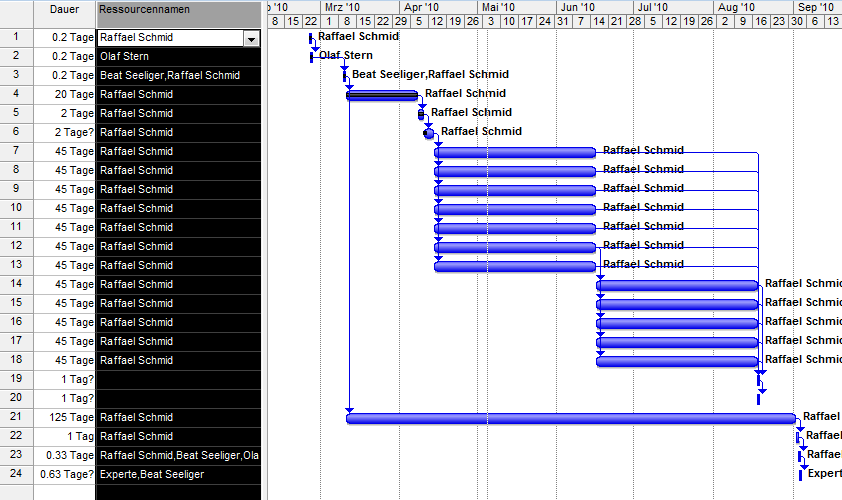
\includegraphics[height=12cm]{orgchart/projectplanning_msproject}
	\caption[Projektplanung MS Project 2007 (stand: 5. Mai 2010)]{Projektplanung MS Project 2007 (stand: 5. Mai 2010)}
\end{figure}
\end{landscape}
Am ende Jeder Phase gibt es einen Meilenstein (Status-Meeting mit Dozenten, Protokoll, Journal der T\"atigkeiten, Problemen und anstehenden Arbeiten.